\documentclass[a4paper,12pt]{article}

% ------------------------------------------------------------
% CAB432 Assignment 3 2026 -- Fractal Farm
% Overleaf-ready scaffold in Nigel's report style.
%
% HOW TO USE
%   * Orange "Your writing" boxes are prompts: every point, decision and
%     piece of evidence to cover in that section. Replace each box with your
%     own prose (the brief requires the report to be drafted by you).
%   * Tables, diagrams, measurements and schemas are factual project
%     artefacts taken from the repository and the live AWS deployment.
%   * Grey "Figure placeholder" boxes mark screenshots still to capture.
%   * Page budget (30 max, excluding references and appendices) is noted
%     at each section heading.
% ------------------------------------------------------------

\usepackage[utf8]{inputenc}
\usepackage[T1]{fontenc}
\usepackage[margin=2cm]{geometry}
\usepackage{array}
\usepackage{booktabs}
\usepackage{tabularx}
\usepackage{longtable}
\usepackage{multirow}
\usepackage{multicol}
\usepackage{enumitem}
\usepackage{graphicx}
\usepackage{float}
\usepackage{caption}
\usepackage{xcolor}
\usepackage{color,colortbl}
\usepackage{sectsty}
\usepackage{hyperref}
\usepackage{fancyhdr}
\usepackage{tikz}
\usepackage[most]{tcolorbox}
\usepackage{amsmath}
\usepackage{adjustbox}
\usetikzlibrary{arrows.meta, positioning, shapes.geometric, fit, backgrounds, calc}

% ------------------------------------------------------------
% Hyperlinks
% ------------------------------------------------------------
\hypersetup{
    colorlinks=true,
    linkcolor=black,
    urlcolor=blue
}

% ------------------------------------------------------------
% Colours (from your earlier report styling)
% ------------------------------------------------------------
\definecolor{sectionColour}{RGB}{15,82,186}
\definecolor{subSectionColour}{RGB}{15,82,186}
\definecolor{subSubSectionColour}{RGB}{0,0,0}
\definecolor{paragraphColour}{RGB}{10,0,20}
\definecolor{mygrey}{RGB}{204,224,255}
\definecolor{softBlue}{RGB}{232,244,255}
\definecolor{softGreen}{RGB}{232,248,240}
\definecolor{softOrange}{RGB}{255,244,232}
\definecolor{softGrey}{RGB}{245,247,250}
\definecolor{softPurple}{RGB}{243,236,255}
\definecolor{qutBlue}{RGB}{0,68,124}
\definecolor{darkText}{RGB}{20,20,20}
\definecolor{mutedText}{RGB}{90,90,90}

% Diagram colours (echo the application's palette)
\definecolor{ffMagenta}{RGB}{214,30,170}
\definecolor{ffCyan}{RGB}{0,160,140}
\definecolor{ffLime}{RGB}{90,160,10}
\definecolor{ffGold}{RGB}{200,150,0}
\definecolor{ffViolet}{RGB}{120,70,200}
\definecolor{ffSky}{RGB}{40,140,200}

% ------------------------------------------------------------
% Section heading styling
% ------------------------------------------------------------
\sectionfont{\color{sectionColour}}
\subsectionfont{\color{subSectionColour}}
\subsubsectionfont{\color{subSubSectionColour}}

% ------------------------------------------------------------
% Page header and footer
% ------------------------------------------------------------
\pagestyle{fancy}
\fancyhf{}
\lhead{CAB432 Assignment 3 2026 -- Fractal Farm}
\rhead{n5453313}
\rfoot{\thepage}
\setlength{\headheight}{15pt}

% ------------------------------------------------------------
% General formatting
% ------------------------------------------------------------
\setlength\parindent{0pt}
\setlength{\parskip}{0.45em}
\setlist{noitemsep, topsep=0.2em}
\renewcommand{\arraystretch}{1.2}

\newcommand{\Hrule}{\rule{\linewidth}{0.5mm}}

\graphicspath{{Images/}}

% \fig{width}{filename}{caption}{label}
\newcommand{\fig}[4]{
\begin{figure}[H]
    \centering
    \includegraphics[width=#1\linewidth]{#2}
    \caption{#3}
    \label{#4}
\end{figure}
}

% Placeholder for screenshots not yet captured
\newcommand{\placeholderfigure}[3]{
\begin{figure}[H]
    \centering
    \fbox{
        \begin{minipage}[c][#1][c]{0.9\linewidth}
            \centering
            \textcolor{mutedText}{\textbf{Figure placeholder:} #2}\\[0.2cm]
            \textcolor{mutedText}{\small Capture at 12\,pt-legible size; zoom the browser (Ctrl +) first.}
        \end{minipage}
    }
    \caption{#2}
    \label{#3}
\end{figure}
}

% ------------------------------------------------------------
% Boxes
% ------------------------------------------------------------
\newtcolorbox{summarybox}{
    colback=softBlue, colframe=sectionColour, arc=1mm, boxrule=0.6pt,
    left=1.5mm, right=1.5mm, top=1.2mm, bottom=1.2mm
}
\newtcolorbox{evidencebox}{
    colback=softGreen, colframe=green!45!black, arc=1mm, boxrule=0.5pt,
    left=1.5mm, right=1.5mm, top=1.2mm, bottom=1.2mm
}
\newtcolorbox{riskbox}{
    colback=softOrange, colframe=orange!70!black, arc=1mm, boxrule=0.5pt,
    left=1.5mm, right=1.5mm, top=1.2mm, bottom=1.2mm
}
\newtcolorbox{schemabox}[1]{
    colback=softGrey, colframe=mutedText, arc=1mm, boxrule=0.4pt,
    left=1.5mm, right=1.5mm, top=1mm, bottom=1mm,
    title={\small #1}, fonttitle=\bfseries, coltitle=white
}

% Writing prompts -- replace each one with your own prose.
\newtcolorbox{yourwriting}[1][]{
    enhanced, breakable,
    colback=softOrange!60, colframe=orange!80!black, arc=1mm, boxrule=0.6pt,
    borderline={0.4pt}{1.2pt}{orange!80!black, dashed},
    left=1.5mm, right=1.5mm, top=1.2mm, bottom=1.2mm,
    title={\small\textbf{Your writing}\ #1}, coltitle=white
}

% Page budget note shown under section headings
\newcommand{\budget}[1]{\hfill{\small\textcolor{mutedText}{\emph{Page budget: #1}}}\par}

% ------------------------------------------------------------
% TikZ styles shared by the diagrams
% ------------------------------------------------------------
\tikzset{
    comp/.style={rectangle, rounded corners=2pt, draw=#1, fill=#1!10, thick,
                 align=center, minimum width=2.9cm, minimum height=1.05cm, font=\small},
    comp/.default=qutBlue,
    store/.style={cylinder, shape border rotate=90, aspect=0.22, draw=#1, fill=#1!10, thick,
                  align=center, minimum width=2.4cm, minimum height=1.2cm, font=\small},
    store/.default=ffLime,
    zone/.style={rectangle, rounded corners=4pt, draw=#1, dashed, thick, inner sep=8pt},
    flow/.style={-{Latex[length=2.2mm]}, thick, #1},
    flow/.default=darkText,
    dflow/.style={-{Latex[length=2.2mm]}, thick, dashed, #1},
    dflow/.default=mutedText,
    lbl/.style={font=\scriptsize, fill=white, inner sep=1pt, text=darkText}
}

% ============================================================
\begin{document}
\pagenumbering{roman}

% ============================================================
% TITLE PAGE (required: title, subtitle, name, ID, AI declaration)
% ============================================================
\thispagestyle{empty}
\begin{titlepage}
    \center
    \vspace*{0.5cm}
    % \includegraphics[width=0.48\linewidth]{qut logo.jpg}
    \vspace{0.4cm}

    \textsc{\Large CAB432 -- Cloud Computing}\\[1.0cm]
    \textsc{\large Assessment 3: Cloud Project}\\[1.0cm]
    \textsc{\large{\textbf{DD - Month - 2026}}}\\[1.0cm]

    \Hrule \\[0.9cm]
    {\Huge \bfseries CAB432 Assignment 3 2026}\\[0.35cm]
    {\Large \bfseries Fractal Farm: a distributed, cached, auto-scaling fractal render farm}\\[0.4cm]
    \Hrule \\[1.1cm]

    \begin{minipage}{0.45\textwidth}
        \begin{flushleft} \Large
            \emph{Author:}\\
            Nigel Jacques\\[0.1cm]
            \emph{Student ID:}\\
            n5453313
        \end{flushleft}
    \end{minipage}
    ~
    \begin{minipage}{0.45\textwidth}
        \begin{flushright} \Large
            \emph{Live system:}\\
            \small\url{https://n5453313-fractal.cab432.com}\\[0.1cm]
            \Large\emph{Source:}\\
            \small\url{https://github.com/Zzort1/fractal-farm}
        \end{flushright}
    \end{minipage}

    \vspace{1.0cm}

    \begin{summarybox}
    \textbf{Declaration of AI use and acknowledgements.}
    \end{summarybox}
    \begin{yourwriting}[-- declaration]
    \begin{itemize}
        \item State which GenAI tools you used and for what (e.g. code generation, debugging, diagram scaffolding, style refinement), and that the report prose is your own.
        \item Acknowledge supplied CAB432 materials and any open-source packages (React, Vite, AWS SDK for JavaScript).
    \end{itemize}
    \end{yourwriting}
\end{titlepage}

% ============================================================
% EXECUTIVE SUMMARY (one page)
% ============================================================
\section*{Executive Summary}
\addcontentsline{toc}{section}{Executive Summary}
\budget{1 page}

\begin{summarybox}
\textbf{At a glance.}
\begin{tabularx}{\linewidth}{>{\bfseries}p{3.6cm} X}
Application & Fractal Farm: interactive deep-zoom explorer for seven fractals, rendered by a cloud worker fleet \\
Why cloud & CPU-heavy, embarrassingly parallel, deterministic and popularity-skewed workload \\
Compute & Three container services on serverless containers: API, render workers, scaling controller \\
Scaling & Metric-based (backlog per worker), scale-out in seconds, scale-to-zero when idle \\
Distribution & Dispatcher-push (load balancer to API) and worker-pull (queue to workers) \\
Caching & Browser HTTP cache, per-instance in-memory LRU, durable object store; edge cache designed \\
Evidence & 1 $\rightarrow$ 6 $\rightarrow$ 8 $\rightarrow$ 0 workers under load; 0 errors; 2.9$\times$ throughput for 3$\times$ workers \\
\end{tabularx}
\end{summarybox}

\begin{yourwriting}[-- one page maximum]
\begin{itemize}
    \item One paragraph: what Fractal Farm is, who it is for, and the problem (render cost, unpredictable demand, repeated views).
    \item One paragraph: architecture in one breath -- stateless API behind a load balancer, queue-fed worker fleet, layered caches, own scaling controller.
    \item Bullet the major decisions: immutable canonical tile URLs; numbers-not-colours tiles; worker-pull with idempotent workers; target tracking on backlog per worker; designing around account restrictions (no managed autoscaling, no managed cache, no CDN).
    \item Name the patterns demonstrated (see Table~\ref{tab:patterns}) and the headline evidence.
    \item One sentence each on what the report covers: agnostic design, AWS realisation, application behaviour, cost and sustainability, reflection.
\end{itemize}
\end{yourwriting}

\newpage
\tableofcontents
\listoffigures
\listoftables
\newpage
\pagenumbering{arabic}

% ============================================================
% 1 INTRODUCTION
% ============================================================
\section{Introduction}
\budget{3 pages}

\subsection{Problem Statement}

\begin{yourwriting}
\begin{itemize}
    \item What a fractal explorer is; why deep zoom is expensive (every pixel iterates up to 4096 times; Lyapunov always runs the full budget).
    \item Why a single machine is a poor fit: measured local 4-worker throughput of 12.8 tiles/s collapses under bursts; demand is spiky (everyone visits at once, then nobody).
    \item Why the cloud: elastic CPU on demand, pay only while rendering, shared durable cache so one user's render serves everyone.
    \item Why this workload is a good vehicle for the unit's concepts: tiles are pure functions of their URL, so caching is safe forever; tiles are independent, so work distributes freely.
\end{itemize}
\end{yourwriting}

\subsection{Requirements}

\begin{table}[H]
\centering
\small
\begin{tabularx}{\linewidth}{>{\bfseries}p{1.2cm} X >{\raggedright\arraybackslash}p{4.2cm}}
\toprule
ID & User story / requirement & Realised by \\
\midrule
FR1 & As an explorer, I can pan and zoom continuously through a fractal. & Canvas tile engine; tile pyramid \\
FR2 & As an explorer, I can choose among seven fractals and change their shape parameters. & Fractal catalogue; canonical parameters \\
FR3 & As an explorer, I can restyle colours instantly without waiting for the cloud. & Client-side colouring of value tiles \\
FR4 & As an explorer, I can open the Julia set of any Mandelbrot point. & Shift-click handler \\
FR5 & As a demonstrator, I can watch queue, workers, caches and scaling live. & Control room over Server-Sent Events \\
\midrule
NFR1 & Scalability: throughput grows with demand; idle cost approaches zero. & Worker fleet 0--8, scaling controller \\
NFR2 & Performance: repeat views are near-instant. & Browser, memory and store cache layers \\
NFR3 & Reliability: no lost or endlessly retried jobs; a crashed worker loses nothing. & Visibility timeout, retries, DLQ, idempotency \\
NFR4 & Security: no anonymous path to unbounded compute; private data stores. & Canonicalisation, input bounds, private bucket \\
NFR5 & Maintainability: same code locally and in the cloud. & Platform adapter layer \\
NFR6 & Cost: run within a student budget. & Scale-to-zero, small tasks, no NAT \\
\bottomrule
\end{tabularx}
\caption{Functional and non-functional requirements.}
\label{tab:requirements}
\end{table}

\begin{yourwriting}[-- requirements discussion]
\begin{itemize}
    \item Explain how you derived the NFRs from the problem (spiky demand $\rightarrow$ NFR1; repeated views $\rightarrow$ NFR2; anonymous public access $\rightarrow$ NFR4).
    \item Note scope boundaries: no user accounts (public explorer), double-precision zoom limit ($\approx 10^{14}$), no edge cache under the account policy.
\end{itemize}
\end{yourwriting}

\subsection{Core Features}

\fig{0.98}{fractal-contact-sheet.png}{The seven fractals at zoom level 1, rendered by the production renderer and coloured by the browser colouring code. Top: Mandelbrot, Julia (Dragon), Multibrot ($d=3$), Burning Ship. Bottom: Tricorn, Newton ($d=3$), Lyapunov (AB).}{fig:contact}

\placeholderfigure{6.5cm}{Main interface: controls (left), viewer (centre), control room (right).}{fig:ui-main}
\placeholderfigure{5.5cm}{Worker tint overlay: each tile coloured by the Fargate task that rendered it.}{fig:ui-workers}
\placeholderfigure{5.5cm}{Control room during scale-out: fleet dots, scaler reason, queue sparkline.}{fig:ui-fleet}

\begin{yourwriting}[-- captions and references]
\begin{itemize}
    \item Reference every screenshot in text (e.g. ``as Figure~\ref{fig:ui-workers} shows\ldots'').
    \item Point out the deliberate split in the UI: \emph{Shape} (changes tile URLs, costs cloud work) versus \emph{Colour} (browser only, free).
\end{itemize}
\end{yourwriting}

\newpage
% ============================================================
% 2 VENDOR-AGNOSTIC ARCHITECTURE
% ============================================================
\section{Vendor-Agnostic Architecture}
\budget{8 pages}

\subsection{Architecture Overview}

\begin{figure}[H]
\centering
\begin{adjustbox}{max width=\linewidth}
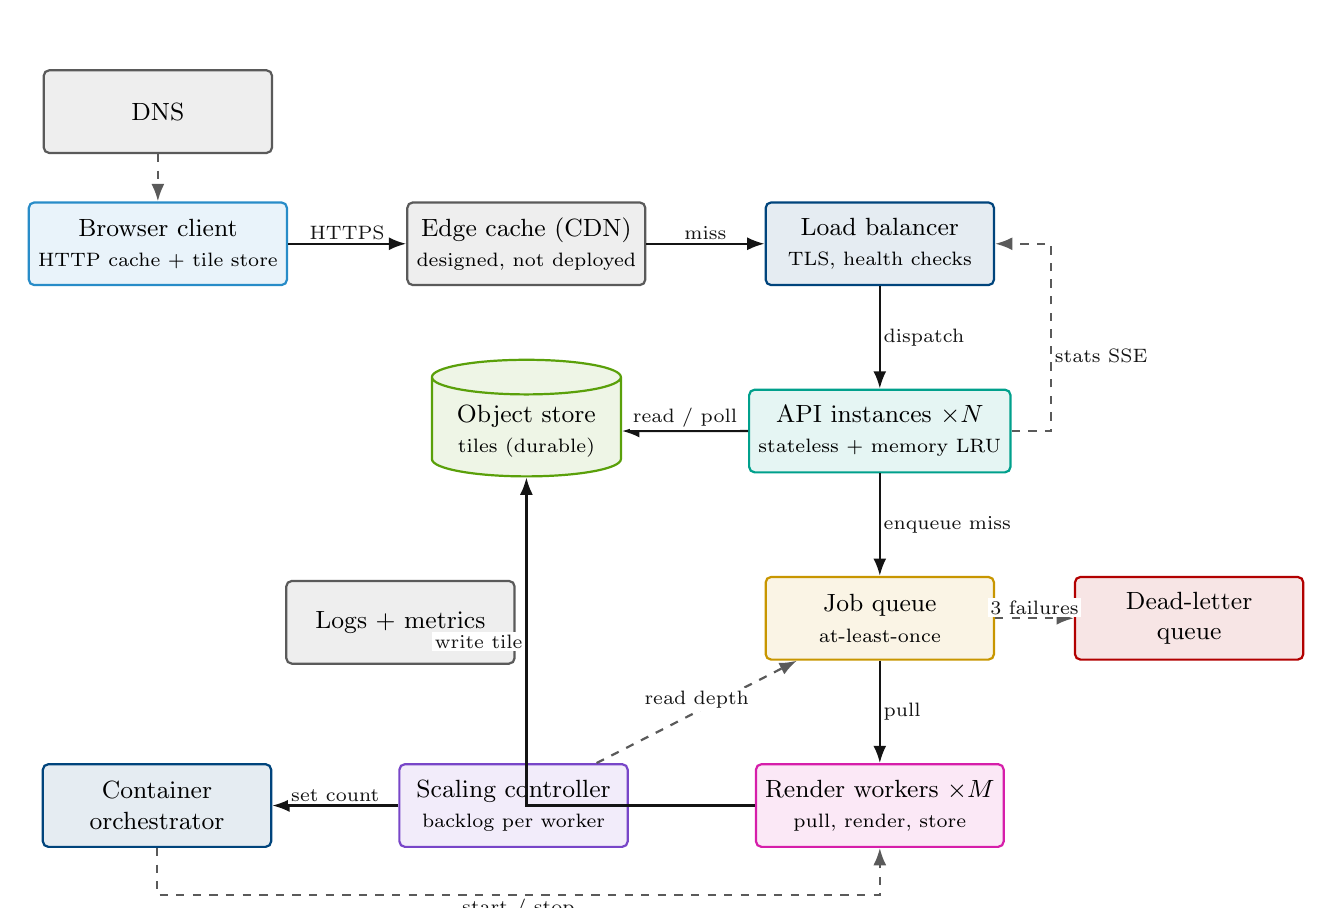
\begin{tikzpicture}[node distance=0.9cm and 1.0cm]
    % Clients and edge
    \node[comp=ffSky] (browser) {Browser client\\\scriptsize HTTP cache + tile store};
    \node[comp=mutedText, right=1.5cm of browser] (edge) {Edge cache (CDN)\\\scriptsize designed, not deployed};
    \node[comp=qutBlue, right=1.5cm of edge] (lb) {Load balancer\\\scriptsize TLS, health checks};

    % API tier
    \node[comp=ffCyan, below=1.3cm of lb] (api) {API instances $\times N$\\\scriptsize stateless + memory LRU};
    \node[store=ffLime, left=1.6cm of api] (obj) {Object store\\\scriptsize tiles (durable)};

    % Async tier
    \node[comp=ffGold, below=1.3cm of api] (queue) {Job queue\\\scriptsize at-least-once};
    \node[comp=red!70!black, right=1.0cm of queue] (dlq) {Dead-letter\\queue};
    \node[comp=ffMagenta, below=1.3cm of queue] (workers) {Render workers $\times M$\\\scriptsize pull, render, store};
    \node[comp=ffViolet, left=1.6cm of workers] (scaler) {Scaling controller\\\scriptsize backlog per worker};
    \node[comp=qutBlue, left=1.6cm of scaler] (orch) {Container\\orchestrator};
    \node[comp=mutedText, below=1.3cm of obj, xshift=-1.6cm] (obs) {Logs + metrics};
    \node[comp=mutedText, above=0.6cm of browser] (dns) {DNS};

    % Flows
    \draw[flow] (browser) -- node[lbl, above]{HTTPS} (edge);
    \draw[flow] (edge) -- node[lbl, above]{miss} (lb);
    \draw[flow] (lb) -- node[lbl, right]{dispatch} (api);
    \draw[flow] (api) -- node[lbl, above]{read / poll} (obj);
    \draw[flow] (api) -- node[lbl, right]{enqueue miss} (queue);
    \draw[flow] (queue) -- node[lbl, right]{pull} (workers);
    \draw[flow] (workers.west) -| node[lbl, pos=0.75, left]{write tile} (obj.south);
    \draw[dflow] (queue) -- node[lbl, above]{3 failures} (dlq);
    \draw[dflow] (scaler) -- node[lbl, above]{read depth} (queue);
    \draw[flow] (scaler) -- node[lbl, above]{set count} (orch);
    \draw[dflow] (orch.south) -- ++(0,-0.6) -| node[lbl, pos=0.25, below]{start / stop} (workers.south);
    \draw[dflow] (dns) -- (browser);
    \draw[dflow] (api.east) -- ++(0.5,0) |- node[lbl, pos=0.2, right]{stats SSE} (lb.east);
\end{tikzpicture}
\end{adjustbox}
\caption{Vendor-agnostic architecture. Solid arrows carry requests and data; dashed arrows carry control, failure and metadata paths.}
\label{fig:agnostic}
\end{figure}

\begin{yourwriting}[-- walk the diagram]
\begin{itemize}
    \item Computing: three roles -- request-facing API (I/O bound), render workers (CPU bound), controller (tiny, singleton). Why separate: different scaling signals and sizes.
    \item Storage: object store for immutable tiles (unstructured blobs, key = URL); per-instance memory cache. Why no database for tiles.
    \item Communication and networking: load balancer (dispatcher-push) at the front, queue (worker-pull) behind; workers have no inbound path at all.
    \item Identity and access: public anonymous reads, but bounded and canonical; services act through least-privilege roles; private bucket.
    \item Other: DNS name stable across replacements; TLS terminated at the load balancer.
\end{itemize}
\end{yourwriting}

\subsection{Design Principles}

\begin{table}[H]
\centering
\small
\begin{tabularx}{\linewidth}{>{\bfseries}p{3.6cm} X X}
\toprule
Principle & Mechanism & Consequence \\
\midrule
Tiles are pure functions & \texttt{tile = f(fractal, params, z, x, y)} & Every cache layer may keep a tile forever; no invalidation logic exists \\
One canonical name per tile & Parameters snapped to fixed steps, sorted, defaults filled; other spellings redirected (301) or rejected (400) & Bounded cache key space; cache-busting attacks impossible \\
Numbers, not colours & Workers return smooth iteration counts; the browser applies palettes & Restyling is free and never fragments the cache \\
Stateless request tier & No session state in API instances & Any instance serves any request; instances are disposable \\
Idempotent workers & Check store before rendering; atomic writes & Duplicate deliveries are harmless \\
Environment-only configuration & Adapter selected by \texttt{PLATFORM} & Identical code locally and in the cloud \\
\bottomrule
\end{tabularx}
\caption{Design principles and their consequences.}
\label{tab:principles}
\end{table}

\begin{yourwriting}
\begin{itemize}
    \item Explain why determinism is the keystone: it is what makes immutable caching and idempotent workers correct.
    \item Trade-off of numbers-not-colours: value tiles are larger than PNGs (Mandelbrot $\approx$ 30\,KB, Lyapunov 4096 $\approx$ 120\,KB gzipped) and the browser does colouring work; in return, palette changes cost zero cloud work.
\end{itemize}
\end{yourwriting}

\subsection{Patterns Selected}

\begin{table}[H]
\centering
\small
\begin{tabularx}{\linewidth}{>{\bfseries}p{3.0cm} >{\raggedright\arraybackslash}p{3.4cm} X}
\toprule
Category & Pattern & Where in Fractal Farm \\
\midrule
Storage & Unstructured store & Tile blobs in the object store, keyed by canonical tile key \\
Caching & In-memory caching & Byte-bounded LRU in every API instance; browser tile store \\
Caching & Edge caching & Immutable \texttt{Cache-Control} honoured by browsers; CDN designed (Section~\ref{sec:limits}) \\
Communication & API gateway / single entry & Load balancer + API as the only public surface \\
Communication & Message queue & Render job queue with dead-letter queue \\
Communication & Polling & 202 + client retry with backoff; queue long polling; store polling for completion \\
Compute & Containers & API, worker and controller as container services on serverless containers \\
Scaling & Metric-based & Worker count tracks backlog per worker \\
Distribution & Dispatcher-push & Load balancer spreading requests over API instances \\
Distribution & Worker-pull & Workers take a job only when free \\
Any of & Event-driven; stateless design; fault tolerance (retries, timeouts, idempotency, coalescing); configuration management; monitoring; garbage collection; WebUI + API + SSE interfaces; public vs private access & Throughout; detailed in Sections~\ref{sec:aws} and~\ref{sec:app} \\
\bottomrule
\end{tabularx}
\caption{Cloud patterns demonstrated (brief requires at least eight).}
\label{tab:patterns}
\end{table}

\begin{yourwriting}
\begin{itemize}
    \item For each pattern, one or two sentences of \emph{why this one} rather than an alternative (e.g. pull vs push to workers: slow heterogeneous jobs; a push dispatcher would need to know worker load).
    \item Make clear which patterns are central (queue, worker-pull, metric scaling, caching) and which are supporting.
\end{itemize}
\end{yourwriting}

\subsection{Scaling Design}

\begin{figure}[H]
\centering
\begin{tcolorbox}[colback=softPurple, colframe=ffViolet, width=0.92\linewidth, arc=1mm, boxrule=0.5pt,
                  title={\small Algorithm 1: target tracking on backlog per worker (every 10\,s)}, fonttitle=\bfseries]
\small
\textbf{Observe:} $v$ = jobs waiting, $f$ = jobs in flight, $d$ = current desired workers\\
\textbf{Policy:} $min$, $max$, target backlog per worker $T$, scale-in cool-down $C$\\[0.3em]
$b \leftarrow v + f$\\
$w \leftarrow \mathrm{clamp}\big(b = 0 \;?\; 0 : \max(1, \lceil b / T \rceil),\; min,\; max\big)$\\
\textbf{if} $w > d$: set desired $\leftarrow w$ immediately; reset cool-down clock \hfill\emph{(out fast)}\\
\textbf{else if} $w = d$: no change; reset cool-down clock\\
\textbf{else}: start clock if not running; \textbf{if} clock $\geq C$: desired $\leftarrow w$ \hfill\emph{(in slowly)}
\end{tcolorbox}
\caption{The scaling decision. Implemented as a pure, unit-tested function.}
\label{fig:algorithm}
\end{figure}

\begin{yourwriting}
\begin{itemize}
    \item Why backlog per worker (not CPU): CPU is pegged at 100\% whether one or fifty jobs wait; backlog per worker maps directly to user wait time ($\approx T \times$ time per tile).
    \item Asymmetry: scale out immediately (cold starts already cost tens of seconds) vs cool-down before scale-in (avoid flapping between bursts).
    \item Scale-to-zero: zero idle cost vs one cold start for the first visitor; mitigations (min = 1 during peak hours, cached popular tiles still served while workers start).
    \item Second scaling dimension: the API tier scales on request rate behind the load balancer (dispatcher-push) -- describe the intended signal and its status.
    \item Why the API waits only 2\,s before answering 202: connections are not held for slow renders; browsers poll with backoff.
\end{itemize}
\end{yourwriting}

\subsection{Asynchronous Workflow}

\begin{yourwriting}
\begin{itemize}
    \item The miss path is asynchronous: enqueue, bounded wait, 202, client polls; the hit path is synchronous.
    \item Request coalescing: concurrent misses for one tile join a single render (measured: 463 coalesced requests in one session).
    \item Completion detection: pub-sub is the ideal; the deployed design polls the store with exponential backoff (100\,ms $\rightarrow$ 2\,s). Quantify the cost: render 6\,ms vs end-to-end 600--750\,ms.
    \item At-least-once delivery and why idempotency makes it safe.
\end{itemize}
\end{yourwriting}

\subsection{Observability Design}

\begin{yourwriting}
\begin{itemize}
    \item Three views: per-service logs (structured JSON), metrics (backlog, backlog per worker, desired/running workers via embedded metric format), and the live control room.
    \item Self-describing tiles: every tile header carries its worker id and render time, so attribution survives every cache layer.
    \item Two vantage points of caching: the browser's (includes its HTTP cache) and the server's (only requests that got past the browser) -- and why both are needed.
\end{itemize}
\end{yourwriting}

\subsection{Security, Reliability and Maintainability}

\begin{yourwriting}
\begin{itemize}
    \item Security: public anonymous reads are bounded (fixed iteration steps, parameter ranges, zoom limit, unknown keys rejected, path-traversal guard in static serving); private bucket; workers unreachable from the internet; least-privilege service roles; TLS 1.3 policy.
    \item Reliability: health-checked instances, visibility timeout redelivery, 3 attempts then DLQ, graceful SIGTERM drain (25\,s) on scale-in, lost-job timeout (120\,s) re-enqueues.
    \item Maintainability: shared core package (one definition of cache keys); adapters; scripts that recreate infrastructure; unit tests on maths and scaling policy.
\end{itemize}
\end{yourwriting}

\subsection{Limitations and Future Work}
\label{sec:limits}

\begin{riskbox}
\textbf{Constraints from the hosting account} (probed, see Appendix~\ref{app:probe}): managed auto-scaling, managed in-memory cache, CDN and pub-sub notification services were not available to the student role.
\end{riskbox}

\begin{yourwriting}
\begin{itemize}
    \item No shared in-memory layer: each API instance has its own LRU, so hit rates fall as instances are added. Future: managed or self-hosted shared cache (and pub-sub for completion).
    \item No edge cache: immutable URLs are CDN-ready; adding one is a configuration change.
    \item Precision: double-precision limit; perturbation theory would be needed beyond.
    \item Abandoned work: jobs for users who left are still rendered (harmless, fills the cache, but costs CPU). Future: drop jobs older than the client's patience.
    \item Single controller: if it stops, the fleet stays at its last size (fail static) until the orchestrator restarts it.
\end{itemize}
\end{yourwriting}

\newpage
% ============================================================
% 3 VENDOR-SPECIFIC IMPLEMENTATION
% ============================================================
\section{Vendor-Specific Implementation (AWS)}
\label{sec:aws}
\budget{7 pages}

\subsection{AWS Architecture}

\begin{figure}[H]
\centering
\begin{adjustbox}{max width=\linewidth}
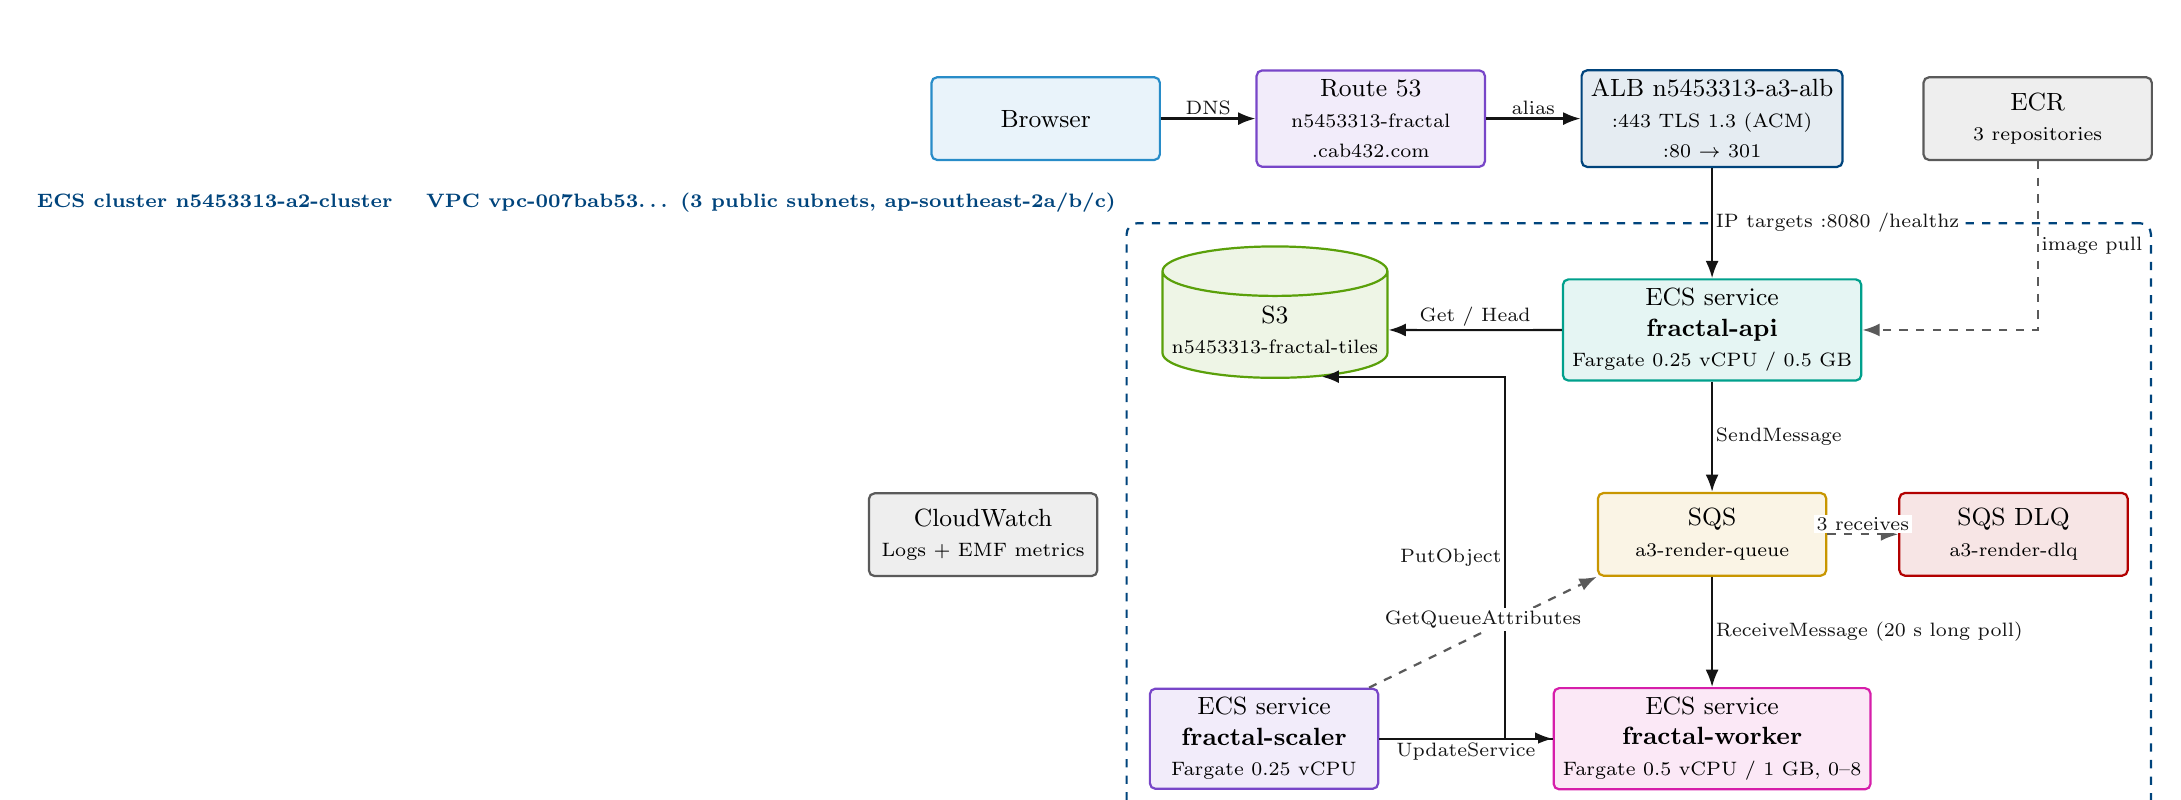
\begin{tikzpicture}[node distance=0.8cm and 0.9cm]
    \node[comp=ffSky] (user) {Browser};
    \node[comp=ffViolet, right=1.2cm of user] (r53) {Route 53\\\scriptsize n5453313-fractal\\\scriptsize .cab432.com};
    \node[comp=qutBlue, right=1.2cm of r53] (alb) {ALB n5453313-a3-alb\\\scriptsize :443 TLS 1.3 (ACM)\\\scriptsize :80 $\rightarrow$ 301};

    \node[comp=ffCyan, below=1.4cm of alb] (api) {ECS service\\\textbf{fractal-api}\\\scriptsize Fargate 0.25 vCPU / 0.5 GB};
    \node[store=ffLime, left=2.2cm of api] (s3) {S3\\\scriptsize n5453313-fractal-tiles};
    \node[comp=ffGold, below=1.4cm of api] (sqs) {SQS\\\scriptsize a3-render-queue};
    \node[comp=red!70!black, right=0.9cm of sqs] (dlq) {SQS DLQ\\\scriptsize a3-render-dlq};
    \node[comp=ffMagenta, below=1.4cm of sqs] (worker) {ECS service\\\textbf{fractal-worker}\\\scriptsize Fargate 0.5 vCPU / 1 GB, 0--8};
    \node[comp=ffViolet, left=2.2cm of worker] (scaler) {ECS service\\\textbf{fractal-scaler}\\\scriptsize Fargate 0.25 vCPU};
    \node[comp=mutedText, left=0.8cm of s3, yshift=-2.6cm] (cw) {CloudWatch\\\scriptsize Logs + EMF metrics};
    \node[comp=mutedText, right=1.0cm of alb] (ecr) {ECR\\\scriptsize 3 repositories};

    \begin{scope}[on background layer]
        \node[zone=qutBlue, fit=(api)(sqs)(worker)(scaler)(s3)(dlq), label={[font=\scriptsize\bfseries, text=qutBlue]north west:{ECS cluster n5453313-a2-cluster \quad VPC vpc-007bab53\ldots\ (3 public subnets, ap-southeast-2a/b/c)}}] {};
    \end{scope}

    \draw[flow] (user) -- node[lbl, above]{DNS} (r53);
    \draw[flow] (r53) -- node[lbl, above]{alias} (alb);
    \draw[flow] (alb) -- node[lbl, right]{IP targets :8080 /healthz} (api);
    \draw[flow] (api) -- node[lbl, above]{Get / Head} (s3);
    \draw[flow] (api) -- node[lbl, right]{SendMessage} (sqs);
    \draw[flow] (sqs) -- node[lbl, right]{ReceiveMessage (20 s long poll)} (worker);
    \draw[flow] (worker.west) -- ++(-0.6,0) |- node[lbl, pos=0.25, left]{PutObject} (s3.south east);
    \draw[dflow] (sqs) -- node[lbl, above]{3 receives} (dlq);
    \draw[dflow] (scaler) -- node[lbl, above]{GetQueueAttributes} (sqs.south west);
    \draw[flow] (scaler) -- node[lbl, below]{UpdateService} (worker);
    \draw[dflow] (ecr) |- node[lbl, pos=0.25, right]{image pull} (api.east);
\end{tikzpicture}
\end{adjustbox}
\caption{AWS implementation (draft). Recreate in draw.io with official AWS icons for submission, keeping the same layout and labels.}
\label{fig:aws}
\end{figure}

\begin{yourwriting}[-- walk the diagram]
\begin{itemize}
    \item Map each agnostic component to its AWS service (Table~\ref{tab:mapping}) and justify the choice.
    \item Network: tasks in public subnets with public IPs so they reach ECR, SQS and S3 without a NAT gateway (cost); security groups (ALB in CAB432SG + default; tasks in default only, which admits only members of itself).
    \item Identity: course-provided execution role (pull images, write logs) and task role (application calls); no credentials in images or code.
\end{itemize}
\end{yourwriting}

\subsection{Service Mapping}

\begin{table}[H]
\centering
\small
\begin{tabularx}{\linewidth}{>{\bfseries}p{3.2cm} >{\raggedright\arraybackslash}p{4.4cm} X}
\toprule
Agnostic role & AWS service & Key configuration \\
\midrule
DNS & Route 53 & A-alias \texttt{n5453313-fractal.cab432.com} $\rightarrow$ ALB \\
Load balancer & Application Load Balancer & Internet-facing, 3 AZs, TLS 1.3 policy, HTTP 301 to HTTPS \\
Certificate & AWS Certificate Manager & DNS-validated via Route 53 \\
Health checking & ALB target group & IP targets, :8080, \texttt{/healthz}, 10\,s interval, 15\,s deregistration \\
Containers & ECS on Fargate & 3 services; images in ECR, tagged by git commit and \texttt{latest} \\
Object store & Amazon S3 & Private; gzip + immutable headers stored with each object \\
Job queue & Amazon SQS & Visibility 60\,s, retention 1\,h, long poll 20\,s \\
Dead-letter queue & Amazon SQS & Redrive after 3 receives; 4-day retention \\
Scaling & Own controller on ECS & \texttt{ecs:UpdateService}; policy in Algorithm 1 \\
Logs and metrics & CloudWatch Logs; EMF & Namespace \texttt{n5453313/FractalFarm} \\
\bottomrule
\end{tabularx}
\caption{Agnostic components and their AWS realisation.}
\label{tab:mapping}
\end{table}

\subsection{Working Within the Account's Constraints}

\begin{table}[H]
\centering
\small
\begin{tabularx}{\linewidth}{>{\bfseries}p{3.6cm} >{\raggedright\arraybackslash}p{3.0cm} X}
\toprule
Wanted service & Probe result & Decision \\
\midrule
Application Auto Scaling & not granted & Own controller: same loop (metric $\rightarrow$ target $\rightarrow$ desired count) via \texttt{ecs:UpdateService}, verified permitted for the task role \\
EC2 Auto Scaling & explicit deny & Containers on Fargate instead of VM groups \\
ElastiCache & explicit deny & Per-instance LRU; completion by store polling instead of pub-sub \\
CloudFront & explicit deny & API serves the web client; immutable headers for browser caching \\
SNS & explicit deny & No push fan-out; polling patterns \\
Log retention & not granted & Logs kept indefinitely (noted as a cost risk) \\
New security groups & denied (A2) & Reuse \texttt{default} and \texttt{CAB432SG} \\
\bottomrule
\end{tabularx}
\caption{Account constraints and the design response.}
\label{tab:constraints}
\end{table}

\begin{yourwriting}
\begin{itemize}
    \item How you discovered these (read-only probe script, exact error text distinguishing ``explicit deny'' from ``no policy allows'').
    \item Why building the controller is not a workaround in spirit: it is the same control loop the managed service runs, now visible and testable; trade-offs (you own its availability; 10\,s tick vs managed alarms).
    \item What you would switch to if the services became available, and why the adapters make that a configuration change.
\end{itemize}
\end{yourwriting}

\subsection{Compute: Fargate Services}

\begin{table}[H]
\centering
\small
\begin{tabularx}{\linewidth}{>{\bfseries}p{2.6cm} p{2.2cm} p{2.0cm} X}
\toprule
Service & Size & Count & Notes \\
\midrule
fractal-api & 0.25 vCPU, 0.5 GB & 1 (min) & Behind ALB; 160\,MB memory cache; serves web client; container health check \\
fractal-worker & 0.5 vCPU, 1 GB & 0--8 & No ports; 30\,s stop timeout for graceful drain \\
fractal-scaler & 0.25 vCPU, 0.5 GB & 1 & Singleton control loop; writes status to S3 and EMF to logs \\
\bottomrule
\end{tabularx}
\caption{ECS services.}
\label{tab:services}
\end{table}

\begin{yourwriting}
\begin{itemize}
    \item Why Fargate over EC2 (no instance management; per-second billing; scale-to-zero of workers is real), and over Lambda for workers (long-lived pull loops; Lambda scaling is excluded by the brief).
    \item Sizing rationale and the measured consequence: 0.5 vCPU renders a 2048-iteration Lyapunov tile in 5.5\,s (p50) -- discuss larger tasks vs more tasks.
    \item Deployment: build multi-stage images, push to ECR, register task definitions, rolling update with health checks.
\end{itemize}
\end{yourwriting}

\subsection{Scaling in Practice}

\begin{figure}[H]
\centering
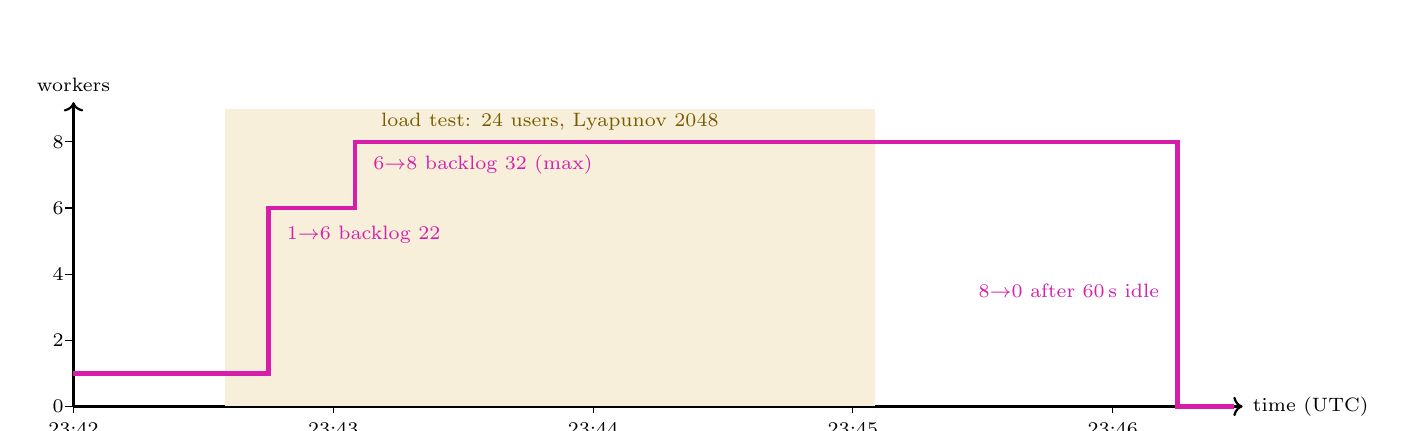
\begin{tikzpicture}[x=0.055cm, y=0.42cm]
    % axes: time in seconds from 23:42:00, workers 0..8
    \draw[->, thick] (0,0) -- (270,0) node[right, font=\scriptsize]{time (UTC)};
    \draw[->, thick] (0,0) -- (0,9.2) node[above, font=\scriptsize]{workers};
    \foreach \y in {0,2,4,6,8} { \draw (-2,\y) -- (0,\y) node[left, font=\scriptsize]{\y}; }
    \foreach \x/\lab in {0/23:42, 60/23:43, 120/23:44, 180/23:45, 240/23:46} {
        \draw (\x,0) -- (\x,-0.2) node[below, font=\scriptsize]{\lab};
    }
    % load window 23:42:35 - 23:45:05
    \fill[ffGold!15] (35,0) rectangle (185,9);
    \node[font=\scriptsize, text=ffGold!60!black] at (110,8.6) {load test: 24 users, Lyapunov 2048};
    % desired workers (step)
    \draw[ultra thick, ffMagenta] (0,1) -- (45,1) -- (45,6) -- (65,6) -- (65,8) -- (255,8) -- (255,0) -- (268,0);
    % annotations
    \node[font=\scriptsize, anchor=west, text=ffMagenta] at (47,5.2) {1$\rightarrow$6 backlog 22};
    \node[font=\scriptsize, anchor=west, text=ffMagenta] at (67,7.3) {6$\rightarrow$8 backlog 32 (max)};
    \node[font=\scriptsize, anchor=east, text=ffMagenta] at (253,3.5) {8$\rightarrow$0 after 60\,s idle};
\end{tikzpicture}
\caption{Desired worker count during the AWS load test (decisions from the scaler log).}
\label{fig:scaling}
\end{figure}

\begin{evidencebox}
\textbf{Measured (2026-10-03, public endpoint).} 164 tiles, 0 errors; time to tile p50 12.8\,s, p95 72\,s; ECS started tasks 10\,s after the first decision; queue drained at 23:45:20 and the fleet reached zero at 23:46:15.
\end{evidencebox}

\begin{yourwriting}
\begin{itemize}
    \item Interpret the timeline: decision latency (one 10\,s tick), task start latency, backlog drain.
    \item Explain the high wait times honestly: target 4 jobs/worker $\times$ 5.5\,s per tile $\approx$ 22\,s; AWS guidance sets the target to acceptable latency $\div$ processing time ($\approx 1$ here). Report the re-tuned run if you perform it.
\end{itemize}
\end{yourwriting}

\subsection{Security Implementation}

\begin{yourwriting}
\begin{itemize}
    \item TLS at ALB (ACM), HTTP redirect; private S3 with public access block; workers have no listener; tasks in \texttt{default} SG reachable only from the ALB's membership.
    \item Input validation (Table~\ref{tab:endpoints} in Appendix): 301 canonical, 400 unknown/invalid, 404 out of range; request body cap 4\,KB on admin endpoints.
    \item Tagging and governance: every resource tagged \texttt{qut-username} and \texttt{purpose = assessment 3} at creation (guardrail-enforced).
    \item Gaps to acknowledge: admin endpoints (cache flush) are unauthenticated in this demo; fix with the existing Cognito pool or ALB authentication.
\end{itemize}
\end{yourwriting}

\newpage
% ============================================================
% 4 APPLICATION IMPLEMENTATION
% ============================================================
\section{Application Implementation}
\label{sec:app}
\budget{6 pages}

\subsection{Data Generated, Processed and Stored}

\begin{table}[H]
\centering
\small
\begin{tabularx}{\linewidth}{>{\bfseries}p{2.8cm} X p{2.6cm} p{2.6cm}}
\toprule
Data & Content & Stored in & Lifetime \\
\midrule
Tile & 32-byte header + 65,536 $\times$ (uint16 value, uint8 class), gzipped & S3; API memory; browser & Indefinite (immutable) \\
Render job & Tile spec + key + enqueue time (JSON) & SQS & $\leq$ 1\,h; DLQ 4 days \\
Scaler status & Policy, depth, counts, reason, history & S3 \texttt{status/} & Overwritten every 10\,s \\
Metrics & Backlog, backlog/worker, desired, running & CloudWatch (EMF) & Per CloudWatch retention \\
Live stats & Counters, rates, history (120\,s) & API memory & Process lifetime \\
User choices & Fractal, params, palette, view & Browser only & Session \\
\bottomrule
\end{tabularx}
\caption{Data in the system.}
\label{tab:data}
\end{table}

\subsection{Messages and Schemas}

\begin{schemabox}{Tile wire format (little-endian)}
\small
\begin{tabularx}{\linewidth}{p{1.6cm} p{1.4cm} X}
offset & bytes & field \\
\midrule
0 & 4 & magic \texttt{FRT1} \\
4 / 6 & 2 + 2 & width, height (256) \\
8 & 4 & render time, ms \\
12 & 20 & worker id (ASCII, NUL-padded) \\
32 & $2N$ & values: 0 = interior, else $1 + \frac{value}{scale}\cdot 65534$ \\
$32+2N$ & $N$ & classes: Newton root index / Lyapunov stability \\
\end{tabularx}
\end{schemabox}

\begin{schemabox}{Render job message (SQS body)}
\footnotesize
\begin{verbatim}
{ "fractal": "lyapunov", "params": { "iter": 2048, "seq": "AB" },
  "paramKey": "iter=2048,seq=AB", "z": 7, "x": 41, "y": 88,
  "key": "lyapunov/iter=2048,seq=AB/7/41/88",
  "enqueuedAt": 1791070965123 }
\end{verbatim}
\end{schemabox}

\begin{schemabox}{Tile request and responses}
\footnotesize
\begin{verbatim}
GET /tiles/julia/5/12/19?cim=0.156&cre=-0.8&iter=512
  200  content-encoding: gzip   cache-control: public, max-age=31536000, immutable
       x-cache: memory | store | render
  202  {"status":"rendering"}   retry-after: 1   cache-control: no-store
  301  location: canonical spelling of the same tile
  400  {"error":"Unknown parameter: bust"}
\end{verbatim}
\end{schemabox}

\begin{yourwriting}
\begin{itemize}
    \item Why a binary format with a header (self-describing across caches; worker attribution without a lookup).
    \item Why JSON for jobs (human-readable in the console; small) and why the job carries the key (workers never recompute it).
    \item Why the server sends gzip and how the browser decodes values and applies palettes.
\end{itemize}
\end{yourwriting}

\subsection{End-to-End Request Flow}

\begin{figure}[H]
\centering
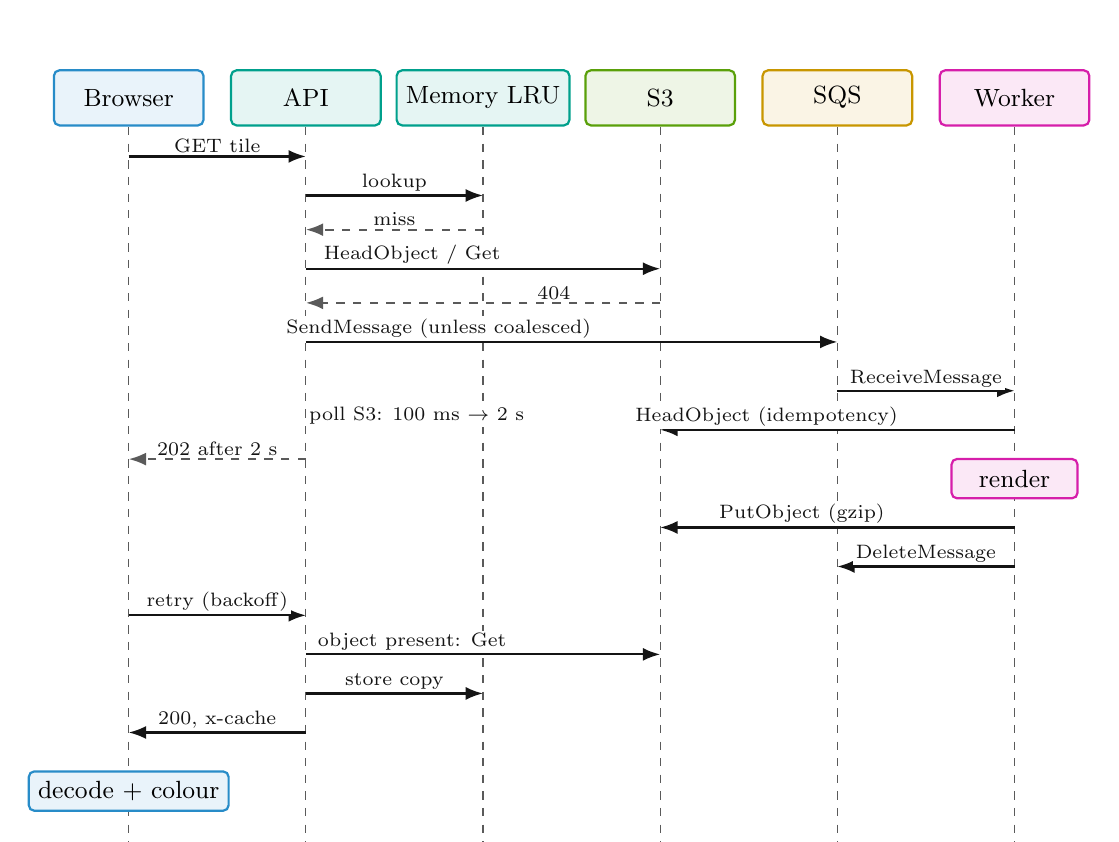
\begin{tikzpicture}[x=2.25cm, y=0.62cm, font=\scriptsize]
    \foreach \nm/\lab/\col [count=\i from 0] in {B/Browser/ffSky, A/API/ffCyan, M/Memory LRU/ffCyan, S/S3/ffLime, Q/SQS/ffGold, W/Worker/ffMagenta} {
        \node[comp=\col, minimum width=1.9cm, minimum height=0.7cm] (\nm) at (\i,0) {\lab};
        \draw[mutedText, dashed] (\i,-0.6) -- (\i,-15.5);
    }
    \draw[flow] (0,-1.2) -- node[lbl, above]{GET tile} (1,-1.2);
    \draw[flow] (1,-2.0) -- node[lbl, above]{lookup} (2,-2.0);
    \draw[dflow] (2,-2.7) -- node[lbl, above]{miss} (1,-2.7);
    \draw[flow] (1,-3.5) -- node[lbl, above, pos=0.3]{HeadObject / Get} (3,-3.5);
    \draw[dflow] (3,-4.2) -- node[lbl, above, pos=0.3]{404} (1,-4.2);
    \draw[flow] (1,-5.0) -- node[lbl, above, pos=0.25]{SendMessage (unless coalesced)} (4,-5.0);
    \draw[flow] (4,-6.0) -- node[lbl, above]{ReceiveMessage} (5,-6.0);
    \draw[flow] (5,-6.8) -- node[lbl, above, pos=0.7]{HeadObject (idempotency)} (3,-6.8);
    \node[comp=ffMagenta, minimum width=1.6cm, minimum height=0.5cm] at (5,-7.8) {render};
    \draw[flow] (5,-8.8) -- node[lbl, above, pos=0.6]{PutObject (gzip)} (3,-8.8);
    \draw[flow] (5,-9.6) -- node[lbl, above]{DeleteMessage} (4,-9.6);
    \node[lbl, right] at (1,-6.5) {poll S3: 100 ms $\rightarrow$ 2 s};
    \draw[dflow] (1,-7.4) -- node[lbl, above]{202 after 2 s} (0,-7.4);
    \draw[flow] (0,-10.6) -- node[lbl, above]{retry (backoff)} (1,-10.6);
    \draw[flow] (1,-11.4) -- node[lbl, above, pos=0.3]{object present: Get} (3,-11.4);
    \draw[flow] (1,-12.2) -- node[lbl, above]{store copy} (2,-12.2);
    \draw[flow] (1,-13.0) -- node[lbl, above]{200, x-cache} (0,-13.0);
    \node[comp=ffSky, minimum width=1.9cm, minimum height=0.5cm] at (0,-14.2) {decode + colour};
\end{tikzpicture}
\caption{Sequence for a tile that misses every cache. Hits end at the memory or S3 step.}
\label{fig:sequence}
\end{figure}

\begin{yourwriting}
\begin{itemize}
    \item Walk the sequence; then the hit paths (memory $\approx$ 2\,ms, S3 $\approx$ 120\,ms measured).
    \item Client side: priority by distance from the view centre, 6 concurrent fetches, ancestor tiles stretched while waiting, polling stops when the tile leaves the view.
    \item Coalescing and the 120\,s lost-job timeout.
\end{itemize}
\end{yourwriting}

\subsection{Error Detection, Handling and Recovery}

\begin{table}[H]
\centering
\small
\begin{tabularx}{\linewidth}{>{\bfseries}p{3.3cm} X X}
\toprule
Failure & Detection & Recovery \\
\midrule
Invalid input & Canonicaliser & 400 / 404 / 301; never enqueued \\
Worker crash mid-render & Message not deleted & Redelivered after 60\,s visibility timeout \\
Poison job & Receive count & Dead-letter queue after 3 receives \\
Duplicate delivery & Tile already in S3 & Acknowledge without rendering \\
Queue unreachable & Receive throws & Worker backs off 0.5\,s $\rightarrow$ 10\,s and continues \\
Lost job & No completion in 120\,s & Pending entry dropped; next request re-enqueues \\
Unhealthy API task & ALB + container health checks & Removed from rotation; ECS replaces \\
Scale-in during render & SIGTERM & Finish within 25\,s grace, else release the job \\
Controller down & ECS service & Restarted; fleet holds last size meanwhile \\
Render thread crash & Thread exit event & Pending renders fail and retry; thread respawned \\
\bottomrule
\end{tabularx}
\caption{Failure modes and responses.}
\label{tab:failures}
\end{table}

\begin{yourwriting}
\begin{itemize}
    \item Pick two failures and narrate them end to end (e.g. scale-in mid-render; poison job to DLQ).
    \item What the user experiences in each case (usually a slightly longer ``rendering\ldots'' border, never an error).
\end{itemize}
\end{yourwriting}

\subsection{Behaviour Under Load and Partial Failure}

\begin{table}[H]
\centering
\small
\begin{tabularx}{\linewidth}{>{\bfseries}p{3.6cm} X X X}
\toprule
Run & Workers & Throughput & Time to tile (p50 / p95) \\
\midrule
Local, Lyapunov 1024, 16 users & 4 & 12.8 tiles/s & 1.79\,s / 2.53\,s \\
Local, Lyapunov 1024, 16 users & 12 & 36.9 tiles/s & 0.63\,s / 0.93\,s \\
AWS, Lyapunov 2048, 24 users & 1 $\rightarrow$ 8 & 1.1 tiles/s & 12.8\,s / 72\,s \\
\bottomrule
\end{tabularx}
\caption{Load test results (0 errors in every run).}
\label{tab:load}
\end{table}

\begin{yourwriting}
\begin{itemize}
    \item Local runs show near-linear scaling (3$\times$ workers, 2.9$\times$ throughput): the workload is parallel.
    \item AWS run: why throughput is lower (0.5 vCPU, 5.5\,s/tile) and what tuning does (target 1, 1 vCPU tasks).
    \item Cache effect under load: hot share 30\% gave 17.7\% hits; browser cache absorbed repeat views (54\% in one session).
    \item Behaviour when a component is unavailable (S3, SQS, a worker, the controller).
\end{itemize}
\end{yourwriting}

\newpage
% ============================================================
% 5 COST AND SUSTAINABILITY
% ============================================================
\section{Cost and Sustainability}
\budget{2 pages}

\subsection{Estimating 50 Concurrent Users}

\begin{table}[H]
\centering
\small
\begin{tabularx}{\linewidth}{>{\bfseries}p{4.2cm} X p{3.0cm}}
\toprule
Quantity & How to obtain & Value \\
\midrule
Tile requests per active user per minute & 15-minute personal session; ALB RequestCount & \emph{measure} \\
Share answered by browser / memory / S3 & Control room ``This browser'' and server panels & \emph{measure} \\
Renders per user per hour & Scaler/worker logs & \emph{measure} \\
Mean render time per tile on 0.5 vCPU & Worker logs (Lyapunov 2048: 5.5\,s) & \emph{per fractal mix} \\
Average workers for 50 users & renders/s $\times$ render time & \emph{compute} \\
New tile storage per month & S3 bucket size growth & \emph{measure} \\
\bottomrule
\end{tabularx}
\caption{Inputs to the 50-user estimate.}
\label{tab:costinputs}
\end{table}

\begin{table}[H]
\centering
\small
\begin{tabularx}{\linewidth}{>{\bfseries}p{4.2cm} X r}
\toprule
AWS service & Calculator input & Monthly (USD) \\
\midrule
Fargate -- API & 1 task $\times$ 0.25 vCPU / 0.5 GB $\times$ 730 h & \\
Fargate -- workers & average tasks $\times$ 0.5 vCPU / 1 GB $\times$ 730 h & \\
Fargate -- scaler & 1 task $\times$ 0.25 vCPU / 0.5 GB $\times$ 730 h & \\
Application Load Balancer & 730 h + LCUs & \\
Amazon S3 & GB-month + PUT/GET/HEAD requests & \\
Amazon SQS & requests (send, receive, delete, attributes) & \\
Route 53 & hosted zone share + queries & \\
CloudWatch Logs & GB ingested + stored & \\
ECR & image storage (3 $\times$ $\approx$ 65\,MB) & \\
\midrule
\textbf{Total} & \emph{public share link from calculator.aws} & \\
\bottomrule
\end{tabularx}
\caption{Cost summary from the AWS Pricing Calculator.}
\label{tab:cost}
\end{table}

\begin{yourwriting}
\begin{itemize}
    \item Show your arithmetic from Table~\ref{tab:costinputs} to the calculator inputs; paste the public share link.
    \item Which costs are fixed (ALB, API, scaler) vs elastic (workers, requests); what scaling does to cost; what scale-to-zero saves overnight.
    \item Cost risks: indefinite log retention; S3 growth (lifecycle rule as garbage collection); abandoned renders.
    \item Sustainability: CPU only runs when someone asked; render-once-serve-many (every cache hit is energy not spent); right-sizing; region choice; client-side colouring moves cheap work to the edge.
\end{itemize}
\end{yourwriting}

\newpage
% ============================================================
% 6 REFLECTION
% ============================================================
\section{Reflection: Learning on My Own}
\budget{2 pages}

\begin{yourwriting}
\begin{itemize}
    \item What you had to research outside the practicals: SQS-based scaling guidance (backlog per instance, acceptable latency $\div$ processing time); ECS service updates as a scaling actuator; CloudWatch Embedded Metric Format; HTTP caching semantics (\texttt{immutable}); Resource Timing to detect browser-cache hits; Fargate task metadata endpoint; graceful SIGTERM handling.
    \item How documentation changed decisions -- concrete examples:
    \begin{itemize}
        \item Probe results $\rightarrow$ rejected ElastiCache/CloudFront/managed scaling; built the controller.
        \item AWS SQS scaling guidance $\rightarrow$ recognised target 4 was too high for 5.5\,s tiles.
        \item Resource Timing $\rightarrow$ fixed a misleading cache display (browser replayed the original \texttt{x-cache}).
        \item Store polling chosen once pub-sub was unavailable; measured its latency cost.
    \end{itemize}
    \item Difficulties: guardrails surfacing as permission errors; Windows CLI quirks (path conversion, CRLF output, credential helper); tag shorthand silently dropping a value -- and what you learned (verify, script everything, read exact error text).
    \item Next iteration: managed scaling and cache if available; latency-based scaling target; larger tasks; second scaling signal for the API; CDN; perturbation-theory deep zoom.
\end{itemize}
\end{yourwriting}

\newpage
% ============================================================
% REFERENCES (not counted)
% ============================================================
\begin{thebibliography}{99}
\addcontentsline{toc}{section}{References}

\bibitem{aws-sqs-scaling} Amazon Web Services. \emph{Scaling policy based on Amazon SQS}. Amazon EC2 Auto Scaling User Guide. \url{https://docs.aws.amazon.com/autoscaling/ec2/userguide/as-using-sqs-queue.html}

\bibitem{aws-ecs-scaling} Amazon Web Services. \emph{Automatically scale your Amazon ECS service}. Amazon ECS Developer Guide. \url{https://docs.aws.amazon.com/AmazonECS/latest/developerguide/service-auto-scaling.html}

\bibitem{aws-dlq} Amazon Web Services. \emph{Using dead-letter queues in Amazon SQS}. \url{https://docs.aws.amazon.com/AWSSimpleQueueService/latest/SQSDeveloperGuide/sqs-dead-letter-queues.html}

\bibitem{aws-emf} Amazon Web Services. \emph{Embedded metric format specification}. Amazon CloudWatch User Guide. \url{https://docs.aws.amazon.com/AmazonCloudWatch/latest/monitoring/CloudWatch_Embedded_Metric_Format_Specification.html}

\bibitem{aws-wa} Amazon Web Services. \emph{AWS Well-Architected Framework}. \url{https://docs.aws.amazon.com/wellarchitected/latest/framework/welcome.html}

\bibitem{aws-fargate-pricing} Amazon Web Services. \emph{AWS Fargate pricing}. \url{https://aws.amazon.com/fargate/pricing/}

\bibitem{mdn-cache} MDN Web Docs. \emph{Cache-Control}. \url{https://developer.mozilla.org/en-US/docs/Web/HTTP/Headers/Cache-Control}

\bibitem{w3c-rt} W3C. \emph{Resource Timing}. \url{https://www.w3.org/TR/resource-timing/}

\bibitem{calc} Amazon Web Services. \emph{AWS Pricing Calculator}. \url{https://calculator.aws/}

\end{thebibliography}
{\small\textcolor{mutedText}{Check each link and add access dates in your referencing style before submission.}}

\newpage
% ============================================================
% APPENDICES (not counted)
% ============================================================
\appendix
\section{Resource Inventory}
\label{app:inventory}

\begin{longtable}{>{\bfseries}p{4.2cm} p{5.2cm} p{6.0cm}}
\caption{Deployed resources (all tagged \texttt{purpose = assessment 3} except the reused cluster).}
\label{tab:inventory}\\
\toprule
Resource & Identifier & Purpose \\
\midrule
\endhead
ECS service & n5453313-fractal-api & Stateless tile API and web client \\
ECS service & n5453313-fractal-worker & Render workers (0--8) \\
ECS service & n5453313-fractal-scaler & Scaling controller \\
ECS cluster (reused) & n5453313-a2-cluster & Hosts all three services \\
ECR repositories & n5453313-fractal-\{api, worker, scaler\} & Container images \\
Task definitions & n5453313-fractal-\{api, worker, scaler\} & Sizes, env, roles, logging \\
S3 bucket & n5453313-fractal-tiles & Tiles and scaler status \\
SQS queue & n5453313-a3-render-queue & Render jobs \\
SQS queue & n5453313-a3-render-dlq & Dead letters \\
ALB & n5453313-a3-alb & Public HTTPS entry \\
Target group & n5453313-a3-api-tg & API tasks, health checks \\
ACM certificate & n5453313-fractal.cab432.com & TLS \\
Route 53 record & n5453313-fractal.cab432.com (A alias) & Stable DNS name \\
CloudWatch log groups & /ecs/n5453313-fractal-\{api, worker, scaler\} & Logs and EMF metrics \\
\bottomrule
\end{longtable}

\section{Permissions Probe}
\label{app:probe}

\begin{table}[H]
\centering
\small
\begin{tabularx}{\linewidth}{>{\bfseries}p{4.5cm} X}
\toprule
Result & Services \\
\midrule
Allowed & ECS, ECR, SQS, S3, DynamoDB, EC2 describe, ELBv2, Route 53, ACM, CloudWatch metrics and dashboards, CloudWatch Logs, Secrets Manager, SSM, Cognito, API Gateway v2, EventBridge Scheduler \\
Not granted & Application Auto Scaling, \texttt{logs:PutRetentionPolicy}, IAM policy listing \\
Explicit deny & EC2 Auto Scaling, ElastiCache, CloudFront, SNS \\
Task role verified & SQS send/receive/delete, S3 get/put/head, \texttt{ecs:UpdateService} \\
\bottomrule
\end{tabularx}
\caption{Read-only probe of the CAB432 account (script \texttt{infra/probe.sh}).}
\label{tab:probe}
\end{table}

\section{API Endpoints}

\begin{table}[H]
\centering
\small
\begin{tabularx}{\linewidth}{>{\ttfamily}p{5.6cm} X}
\toprule
\normalfont\bfseries Endpoint & \textbf{Purpose} \\
\midrule
GET /tiles/\{f\}/\{z\}/\{x\}/\{y\}?\ldots & Tile: 200, 202, 301, 400, 404 \\
GET /api/fractals & Fractal catalogue \\
GET /api/stats & One stats snapshot \\
GET /api/events & Stats stream (Server-Sent Events, 1\,Hz) \\
POST /api/cache/flush & Empty the instance memory cache (demo) \\
POST /api/workers & Local mode only: set worker count \\
GET /healthz & Load balancer health check \\
GET /* & Built web client (hashed assets immutable) \\
\bottomrule
\end{tabularx}
\caption{HTTP interface.}
\label{tab:endpoints}
\end{table}

\section{Reproducing the Deployment}

\begin{tabularx}{\linewidth}{>{\ttfamily}p{5.8cm} X}
\toprule
\normalfont\bfseries Script & \textbf{Effect} \\
\midrule
infra/probe.sh & Read-only permissions probe \\
infra/stage2-storage-queue.sh & Bucket, queue, DLQ (tagged) \\
infra/stage3-images.sh & ECR repositories; build and push images \\
infra/stage3-ecs.sh & Log groups, task definitions, worker service \\
infra/stage4-public.sh & Certificate, ALB, listeners, DNS, API service \\
infra/stage5-scaler.sh & Scaler service; rolling update of all services \\
scripts/loadtest.js & Load generator used for Table~\ref{tab:load} \\
\bottomrule
\end{tabularx}

\end{document}
